
\documentclass[lettersize,journal]{IEEEtran}
\usepackage{amsmath,amssymb,amsfonts}
\usepackage{array}
\usepackage{booktabs}
\usepackage{multirow}

\usepackage{algorithm}
\usepackage{algorithmic}

\usepackage{graphicx}
\usepackage[cmyk]{xcolor}
\usepackage{textcomp}
\usepackage{soul}

% IEEE recommended sub-figures (use \subfloat, not subfigure environment)
% Use roman (same as main text) for sub-figure captions/labels
\usepackage[caption=false,font=normalsize,labelfont=rm,textfont=rm]{subfig}

\usepackage{url}
\usepackage{verbatim}
\usepackage{cite}
\usepackage{stfloats}

% CJK + hyperlinks/cleveref (order matters: hyperref -> cleveref)
\usepackage{xeCJK}
\usepackage{hyperref}
\usepackage{cleveref}


\hyphenation{op-tical net-works semi-conduc-tor IEEE-Xplore}
% updated with editorial comments 8/9/2021

\begin{document}

\title{KAMT: Knowledge-Augmented multi-modal learning based AD and relevant dementia(ADRD) diagnosis}



\author{IEEE Publication Technology,~\IEEEmembership{Staff,~IEEE,}
        
}

% The paper headers
\markboth{Trans}%
{Author \MakeLowercase{\textit{et al.}}: KAMTT}



\maketitle

\begin{abstract}
        For precision diagnosis, the model performance of deep learning approaches has an over-reliance on sample size and data quality.
        In this case, domain knowledge has played an essential role in enhancing the credibility and reliability of deep learning approaches, especially in precision medicine applications. Neuroimage samples and clinical metadata have been employed to conduct precision diagnostic models for ADRD and cognitive impairment. For the textual modality associated with AD and dementia, the semantic relations between biomedical entities could be applied as domain knowledge to guide the learning of deep neural networks. Under the MML framework, this work proposes the KAMT architecture to enhance prediction accuracy and credibility in ADRD diagnosis.   
        
\end{abstract}

\begin{IEEEkeywords}
	Clinical knowledge, multi-omics integration, ADRD diagnosis.
\end{IEEEkeywords}

\section{Introduction}
\label{sec:introduction}

    \textcolor{blue}{\IEEEPARstart{A}{ssessment} of brain diseases has become an important topic in precision medicine. For neurodegenerative diseases such as Parkinson's disease (PD) and Alzheimer's disease (AD), multimodal deep learning integrating diverse features has gradually become the mainstream approach in this field \cite{qiu2022multimodal,zhang2026multimodalpd}. Recent advanced frameworks have even attempted to ground diagnostic decisions in localized anatomy and clinical variables to improve transparency \cite{lin2025adlip,wood2026align}. Specifically, practical diagnostic pipelines typically involve extracting baseline information from Electronic Health Records (EHR)\cite{rajkomar2018scalable}, tracking the dynamic changes of clinical scales within Biomarkers (BM)\cite{marek2011parkinson}, and utilizing 3D-CNNs \cite{basaia2019automated} to preprocess Magnetic Resonance Imaging (MRI) for capturing localized microstructural patterns.}

    However, lacking prior guidance on underlying pathological mechanisms, purely data-driven models heavily rely on isolated numerical computations and image feature extraction. By ignoring the critical semantic associations between biomedical entities in medical records, these approaches suffer from severe overfitting and performance degradation\cite{lu2021knowledge} when applied to multi-center clinical cohorts with heterogeneous feature distributions.

    \textcolor{blue}{With efficient representations, the Knowledge-Augmented learning scheme could provide a way to improve the model performance as well as model explainability. It is noted that the quality of knowledge representations determines the prediction accuracy and model generalization ability in precision medicine \cite{chandak2023building}.}  \textcolor{blue}{Motivated by established works about large-scale Clinical knowledge graphs including SPOKE \cite{morris2023spoke} and PharmKG \cite{zheng2021pharmkg}, this work develops the dementia-specific knowledge graphs by extracting complicated causal relations between biomedical ontology that are associated with brain disease and cognitive decline.}

    \textcolor{blue}{Knowledge-augmented neural network learning architecture is another essential perspective in obtaining reliable predictions} from multimodal data. \textcolor{blue}{With external knowledge, Relational knowledge graphs were constructed to capture causal relations for biomedical entities that are associated with dementia and cognitive decline. For neurological disorders, essential ontologies such as vascular dynamics and immune regulation have been encoded in the triplets in large-scale biomedical KG \cite{zhao2026kgt,sim2024gtad}.}
    
\begin{itemize}
    \item High-quality knowledge representations have been extracted and exploited in disease prediction;
    \item Clinical knowledge-augmented learning scheme has been proposed to integrate augmented knowledge representations and multi-modal learning;
    \item  For dementia and cognitive impairment, clinic knowledge has been extracted as triplets and incorporated into multimodal learning network;
    \item External knowledge source was introduced to obtain high-quality domain knowledge in the diagnostic of ADRD, with the proposed X-KD strategy.
\end{itemize}




\section{Related Works}

\subsection{Multimodal Deep Learning for Dementia Diagnosis}

    Multimodal deep learning approaches have been widely used for assessing Alzheimer's disease and related dementia(ADRD) by jointly modeling clinical text and imaging phenotypes \cite{jin2026multimodal}. While attention-based fusion has improved representation capacity, purely data-driven models can still exhibit distribution shift and reduced generalization across sites/cohorts with heterogeneous acquisition protocols and feature distributions \cite{abugabah2025intelligent}. In addition, without explicit mechanistic priors, these models may rely on spurious within-modality correlations and underutilize clinically meaningful semantic links between medical entities and cognitive outcomes.

\subsection{Knowledge-Guided Multimodal Fusion Frameworks}

    Clinical knowledge graphs offer structured priors that can support multimodal learning. It is noted that directly incorporating large-scale, general-purpose KGs may introduce biological noise and dilute task-relevant signals. In contrast, domain-specific graphs built from local records can better match the target cohort yet often lack ontology breadth and transferability. These trade-offs motivate task-adaptive relational diagnostic KGs that balance specificity with external coverage.


    Multiple knowledge-enhanced multimodal models still follow a shallow fusion strategy, treating KG embeddings as independent vectors that are concatenated with image/text features near the output \cite{chen2023knowledge}, which can limit how knowledge shapes intermediate learning and cross-modal alignment. Recent diagnostic models therefore increasingly use Transformer-style self-/cross-attention to adaptively weight and align heterogeneous representations \cite{vaswani2017attention,kyritsis2025transformerfusionad,li2024hammf,du2025vitadreview,chen2026federatedvitad}. In this work, we address the gap between shallow knowledge injection and fine-grained fusion by introducing knowledge-augmented features into the cross/self-attention module, allowing KG information to act as an implicit constraint that guides multimodal representation learning.

    
\section{Clinic-guided KAMT Method}

    \textcolor{blue}{In precision diagnosis of brain diseases, knowledge graph embedding (KGE) methods aim to encode biomedical entities and their relations into a low-dimensional semantic space.}
    \textcolor{blue}{Specifically, the KGE method learns low-rank entity representations by scoring observed triplets higher than corrupted ones. Representative models include TransE\cite{bordes2013translating}, DistMult, ComplEx\cite{trouillon2016complex}, and RotatE\cite{sun2019rotate}. For digital medicine, multi-hop reasoning is required.}

    To address this gap, this work proposes a controlled relation graph refinement paradigm: task-specific multimodal seeds have been extracted and topological refinement has been conducted to build a dementia-oriented relational KG (DemRKG), in order to learn global entity representations.

\begin{comment}
The overall refinement and construction pipeline is illustrated in \cref{fig:dementia_hkg_flow}.

\begin{figure}[htbp]
    \centering
    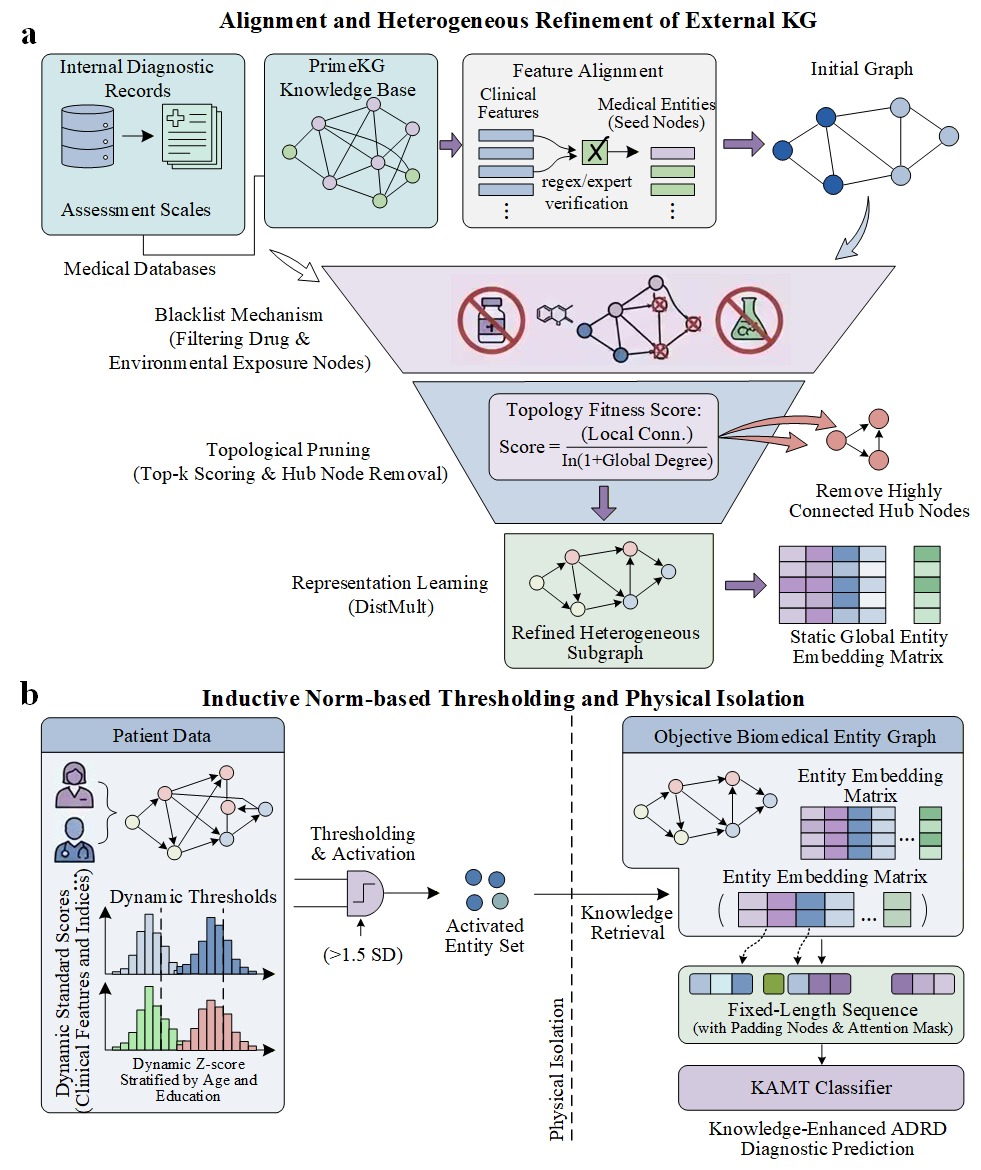
\includegraphics[width=\linewidth]{Figures/DementiaHKG流程图-EN.png}
    \caption{The construction, refinement, and patient-specific activation pipeline of DemRKG. (a) Alignment and heterogeneous refinement of the external KG, illustrating the topological pruning and DistMult representation learning. (b) Inductive norm-based thresholding and physical isolation for objective patient sequence generation.}
    \label{fig:dementia_hkg_flow}
\end{figure}
\end{comment}

\subsection{Refinement of DemRKG}

\subsubsection{Retrieval and Alignment of Medical Entities}

    We first align internal clinical features in $\mathcal{F}$ to PrimeKG nodes $\mathcal{V}$ via a mapping $M: \mathcal{F} \rightarrow \mathcal{V}$. To improve matching precision, we extract core medical roots to build regular expressions and conduct fuzzy matching within constrained disease/phenotype subsets; final mapping rules are verified by experts. This yields a seed set $\mathcal{S}=\mathcal{S}_{\mathrm{core}}\cup\mathcal{S}_{\mathrm{clinical}}$, where $\mathcal{S}_{\mathrm{core}}$ injects clinically agreed key pathology nodes (e.g., Alzheimer's disease and APOE).

\subsubsection{Dynamic Pruning Based on Node Degrees}

    From $\mathcal{S}$, we expand a 2-hop neighborhood to capture multistep associations. Following network-medicine practice, we emphasize protein--protein interactome (PPI) connections to contextualize disease mechanisms \cite{barabasi2011network,cheng2019network}. To suppress non-specific hub nodes, a specificity score was defined to penalize global degree, formulated by Eq.(\ref{eq:spec-score}).

    \begin{equation}
        Score(w) = \frac{L(w)}{\ln(1 + G(w))}
        \label{eq:spec-score}
    \end{equation}

    where $L(w)$ denotes the number of links between node $w$ and the current subgraph, and $G(w)$ is its global degree in PrimeKG. We then perform score-based $\mathrm{Top}\text{-}k$ truncation with $k=5$ for ADNI/NACC and $k=6$ for AIBL/PPMI.

\subsubsection{Construction of Graph Sequences}

    To avoid information leakage, we retain only objective entities for KG activation. Using cognitively normal (NC) subjects from the training set as dynamic normative baselines, each clinical index $f_{i,k}$ was standardized according to Eq.(\ref{eq:zscore_calc}).
    
    \begin{equation}
        Z_{i, k} = \frac{f_{i, k} - \mu_{\mathrm{age}, \mathrm{edu}}}{\sigma_{\mathrm{age}, \mathrm{edu}}}
    \label{eq:zscore_calc}
    \end{equation}

    Empirically, if $|Z_{i,k}|>1.5$, we activate (map) the corresponding abnormal phenotype node.

    Given refined triplets $\mathcal{T}$ from DemRKG, this study pre-trains KG embeddings in $\mathbb{R}^d$ with negative sampling by corrupting entities. With the margin $\gamma=1.0$, the loss function of KGE is defined by Eq.(\ref{eq:margin_loss}).
    
    \begin{equation}
        \mathcal{L} = \sum_{(h, r, t) \in \mathcal{T}} \sum_{(h, r, t') \in \mathcal{T}'} \max(0, \gamma - f(h, r, t) + f(h, r, t'))
        \label{eq:margin_loss}
    \end{equation}

    In this case, entity embeddings $\mathbf{E} \in \mathbb{R}^{|\mathcal{V}| \times d}$ and relation embeddings $\mathbf{R} \in \mathbb{R}^{|\mathcal{R}| \times d}$ were determined. For each patient, we build $\mathbf{X}_{KG} \in \mathbb{R}^{L_{kg} \times d}$ by indexing $\mathbf{E}$, and feed it to the cross-attention module with mask $\mathbf{m}$ to implicitly constrain knowledge injection.

\subsection{Multimodal Feature Space Division}

    \subsubsection{Textual representations of clinic metadata}
    
    A modality split mapping function $f_{\mathrm{split}}$ projects the cleaned clinical feature set $\mathcal{D}_{\mathrm{clean}}$ into two independent subspaces:
    
    \begin{equation}
        \mathcal{M}_{\mathrm{EHR}}, \mathcal{M}_{\mathrm{BM}} = f_{\mathrm{split}}(\mathcal{D}_{\mathrm{clean}})
        \label{eq:modality_split}
    \end{equation}

    The static background modality $\mathcal{M}_{\mathrm{EHR}}$ encodes prior attributes (e.g., demographics and basic medical history). The dynamic phenotype modality $\mathcal{M}_{\mathrm{BM}}$ represents disease-specific clinical scales and biological states.

% \subsubsection{Clinical Text Feature Extraction}
    
    Independent Multi-Layer Perceptron (MLP) encoders map the split text modality features into a shared latent representation space \cite{wang2024unity}. For a text feature vector $\mathbf{x} \in \mathbb{R}^{d_{in}}$, continuous linear transformations are executed via a two-layer perceptron:
    
    \begin{equation}
    \mathbf{h} = \text{ReLU}(\text{BN}(\mathbf{W}_1 \mathbf{x} + \mathbf{b}_1))
    \label{eq:MLP_1}
    \end{equation}
    \begin{equation}
    \mathbf{z} = \text{ReLU}(\text{BN}(\mathbf{W}_2 \text{Dropout}(\mathbf{h}) + \mathbf{b}_2))
    \label{eq:MLP_2}
    \end{equation}

    where $\mathbf{W}_1$ and $\mathbf{W}_2$ are weight matrices, and $\mathbf{b}_1$ and $\mathbf{b}_2$ denote bias terms. Batch Normalization ($\text{BN}$) stabilizes the data distribution, and $\text{Dropout}$ mitigates overfitting. The output $\mathbf{z} \in \mathbb{R}^{d_{embed}}$ serves as the unified embedding vector.


\subsubsection{MRI Image Feature Extraction}
    
    For neuroimaging, the 3D-CNN encoder extracts spatial voxel associations $\phi_{\mathrm{img}}$ from structural MRI data \cite{wen2020convolutional}. The input volume ($depth \times height \times width$) first undergoes center cropping:
    \begin{equation}
        I_{crop} = I [d_{s}:d_{e}, h_{s}:h_{e}, w_{s}:w_{e}]
        \label{eq:center_crop}
    \end{equation}

    For visual features, 3D convolution kernels extract high-order morphological representations \cite{tran2015c3d}. At the 3D spatial position $(x, y, z)$, the $k$-th feature map is computed as:
    
    \begin{equation}
        v_{x,y,z}^{k} = \sigma \left( \sum_{i,j,l} w_{i,j,l}^{k} \cdot I_{x+i, y+j, z+l} + b^k \right)
        \label{eq:3dcnn}
    \end{equation}

    where $I$ represents the 3D MRI data, and $\sigma$ is the nonlinear activation function. Flattening and linear projection operations align the high-dimensional image features with the text modalities:
    \begin{equation}
        Z_{img} = \mathrm{ReLU}(\mathbf{W}_{f} \cdot \mathrm{Flatten}(v) + \mathbf{b}_f)
        \label{eq:mri_projection}
    \end{equation}

    The representation vector $Z_{img}$ functions as the unified image input. 

\subsection{Knowledge-Augmented Multimodal Synergistic Interaction}

    The KAMT method has coupled modality-aware knowledge retrieval with an energy-constrained refinement pathway, as summarized in \cref{fig:KAMT_framework}.

    \begin{figure*}[!t]
        \centering
        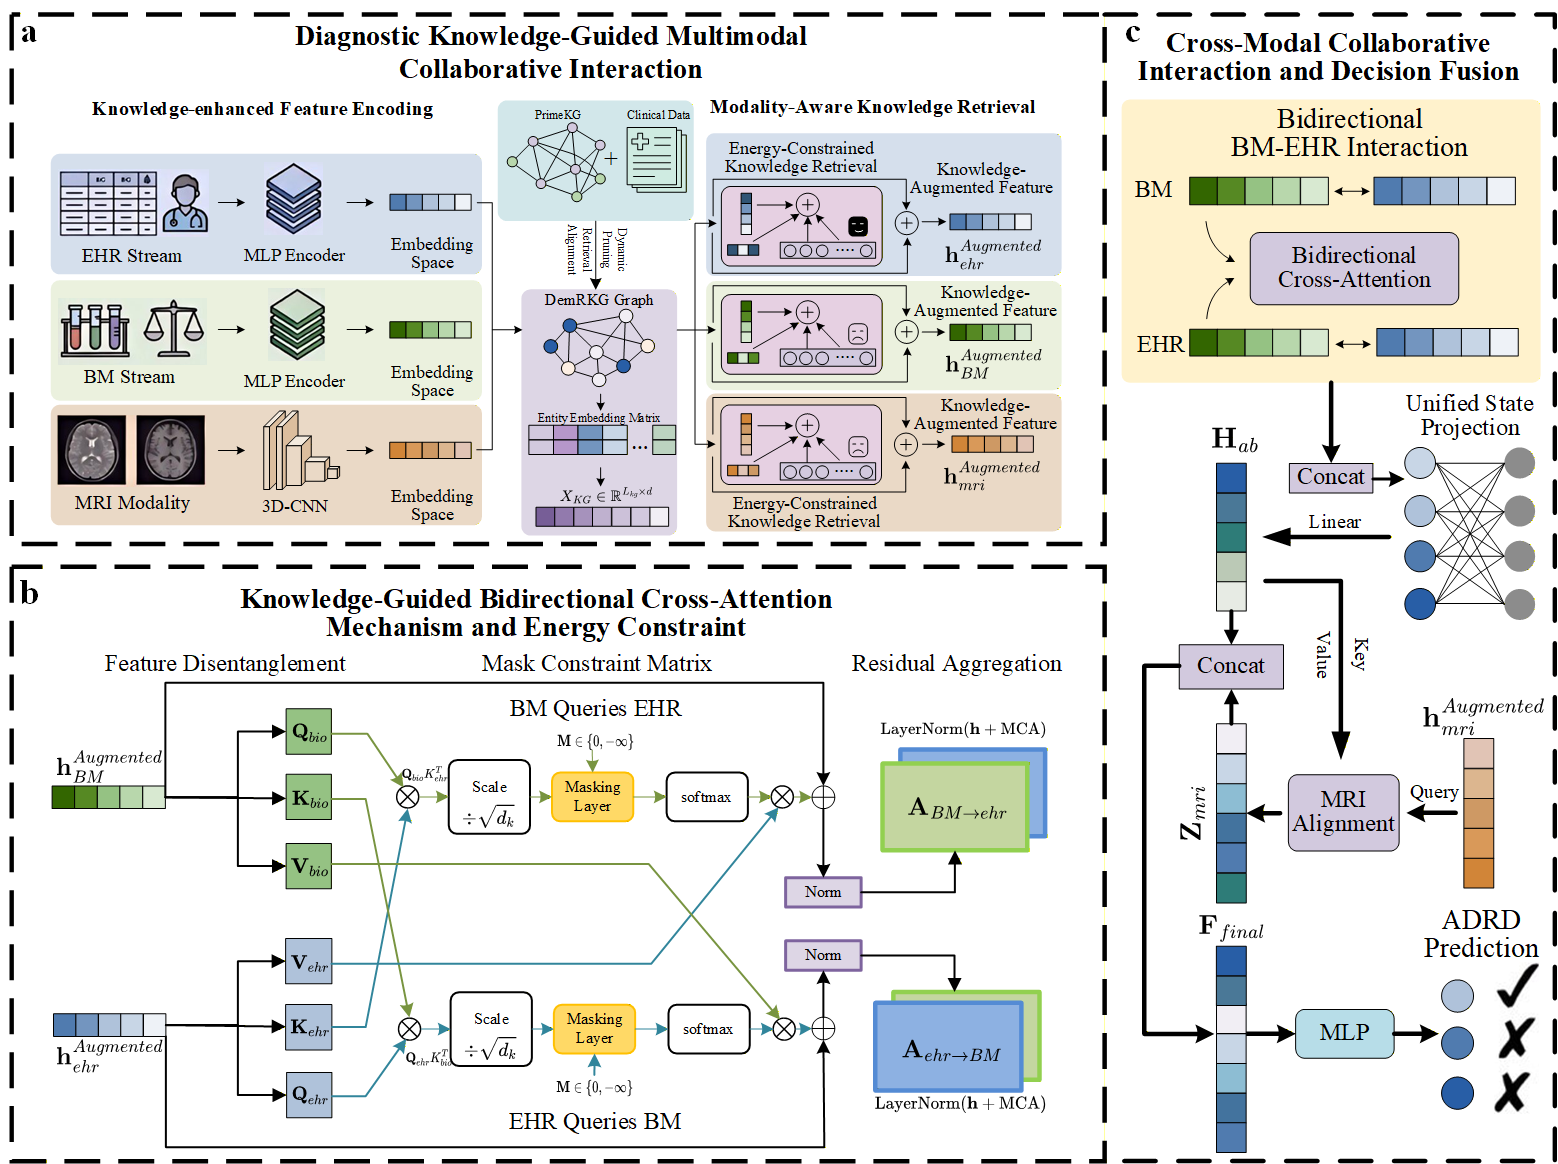
\includegraphics[width=\textwidth]{Figures/KAMT-Trans框架图.png}
        \caption{Overall architecture of KAMT. (a) Knowledge-Augmented encoding and modality-aware retrieval from KG sub-graphs. (b) Masked cross-attention for knowledge injection and the proposed energy-constrained refinement. (c) BM-EHR collaboration guides MRI alignment; the final prediction is made from the fused low-level state and aligned MRI representation.}
        \label{fig:KAMT_framework}
    \end{figure*}

    %\textcolor{purple}{Roles and functions of energy-constrained refinement pathway are still unclear.}
    This energy-constrained refinement pathway acts as a structural regularizer that filters clinical noise and injects reliable medical priors from DemRKG, which prevents overfitting on limited data.

\subsubsection{Dynamic Constraints and Prior Guidance of the Knowledge Graph}

    For each modality $m$, the corresponding network nodes are projected into a continuous space to form a modality-aware manifold dictionary:
    
    \begin{equation}
        \mathcal{M}_{kg}^{(m)} = \mathrm{span} \{ \mathbf{h}_{kg, m}^{(1)}, \mathbf{h}_{kg, m}^{(2)}, \dots, \mathbf{h}_{kg, m}^{(N)} \} \subset \mathbb{R}^d.
        \label{eq:manifold_dict}
    \end{equation}

    Given the modality feature $\mathbf{h}_m$, KAMT refines it by minimizing an energy with a data term and a KG prior term:
    
    \begin{equation}
        \mathbf{h}_m^* = \arg\min_{\mathbf{h}} \Big( \| \mathbf{h} - \mathbf{h}_m \|^2 + \lambda \, \mathcal{D}(\mathbf{h}, \mathcal{M}_{kg}^{(m)}) \Big),
        \label{eq:energy_min}
    \end{equation}

    where $\mathcal{D}(\mathbf{h}, \mathcal{M}_{kg}^{(m)})$ measures the distance between $\mathbf{h}$ and the modality-specific KG span (implemented via the residual to its projection onto $\mathcal{M}_{kg}^{(m)}$).

\subsubsection{Modality-Specific Knowledge Retrieval}

    Each modality is encoded to $\mathbf{h}_m \in \mathbb{R}^{B \times 1 \times d}$. Relevant KG nodes are activated, padded to length $N$, and masked by $\mathbf{M} \in \{0, -\infty\}^{B\times N}$. The masked cross-attention retrieves the knowledge response, described by Eq.(\ref{eq:knowledge_response}).
    
    \begin{equation}
        \mathbf{z}_{m}^{kg} = \mathrm{softmax}\left( \frac{(\mathbf{h}_m \mathbf{W}_m^Q) (\mathbf{H}_{kg}^{(m)} \mathbf{W}_m^K)^\top}{\sqrt{d_k}} + \mathbf{M} \right) (\mathbf{H}_{kg}^{(m)} \mathbf{W}_m^V).
        \label{eq:knowledge_response}
    \end{equation}

    Clinical knowledge was injected by residual fusion: 
    \begin{equation}
    \mathbf{h}_m^{Augmented} = \mathrm{LayerNorm}(\mathbf{h}_m + \mathbf{z}_{m}^{kg})
    \end{equation}

\subsubsection{Knowledge-Augmented Text Modality Interaction}

    Using the augmented BioMarker and EHR features, KAMT performs bidirectional cross-attention:
    
    \begin{equation}
        \begin{aligned}
        \mathbf{A}_{BM \rightarrow ehr} &= \mathrm{LayerNorm}(\mathbf{h}_{BM}^{Augmented} + \mathrm{MCA}(\mathbf{Q}_{BM}, \mathbf{K}_{ehr}, \mathbf{V}_{ehr})), \\
        \mathbf{A}_{ehr \rightarrow BM} &= \mathrm{LayerNorm}(\mathbf{h}_{ehr}^{Augmented} + \mathrm{MCA}(\mathbf{Q}_{ehr}, \mathbf{K}_{BM}, \mathbf{V}_{BM})).
        \end{aligned}
        \label{eq:bidirectional_mca}
    \end{equation}

    The low-level health state is obtained by a lightweight fusion:
    
    \begin{equation}
        \mathbf{H}_{ab} = \mathrm{Linear}\Big(\big[\mathrm{Squeeze}(\mathbf{A}_{BM \rightarrow ehr}) \parallel \mathrm{Squeeze}(\mathbf{A}_{ehr \rightarrow BM})\big]\Big).
        \label{eq:hab_def}
    \end{equation}


    The augmented MRI features were aligned using $\mathbf{H}_{ab}$ as Key and Value vectors.
    
    \begin{equation}
        \mathbf{Z}_{mri} = \mathrm{LayerNorm}(\mathbf{h}_{mri}^{Augmented} + \mathrm{MCA}(\mathbf{Q}_{mri}, \mathbf{H}_{ab}, \mathbf{H}_{ab})).
        \label{eq:mri_alignment}
    \end{equation}

    The joint latent representation concatenates only $\mathbf{H}_{ab}$ and $\mathbf{Z}_{mri}$:

    \begin{equation}
    \mathbf{F}_{final} = [ \mathrm{Squeeze}(\mathbf{H}_{ab}) \parallel \mathrm{Squeeze}(\mathbf{Z}_{mri}) ].
    \label{eq:final_fusion}
    \end{equation}

    Subsequently, $\mathbf{F}_{final}$ was fed into an MLP classifier for diagnosis.


    The fused representation $\mathbf{F}_{final}$ was mapped to logits $z_{i,c}$ and converted to class probabilities via Softmax, described as follows.
    
    \begin{equation}
        \hat{y}_{i,c} = \frac{\exp(z_{i,c})}{\sum_{j=1}^{C} \exp(z_{i,j})}
        \label{eq:softmax}
    \end{equation}

    We optimize a $C$-class cross-entropy loss over a batch of size $B$:
    
    \begin{equation}
        \mathcal{L}_{CE} = - \frac{1}{B} \sum_{i=1}^{B} \sum_{c=1}^{C} y_{i,c} \log(\hat{y}_{i,c})
        \label{eq:cross_entropy}
    \end{equation}

    where $y_{i,c}$ is the one-hot ground-truth label. Following Adam \cite{kingma2014adam}, we apply $L_2$ regularization to learnable parameters $\theta$, yielding the objective:
    
    \begin{equation}
        \mathcal{L}_{KAMT} = \mathcal{L}_{CE} + \lambda \sum_{w \in \theta} w^2
        \label{eq:total_loss}
    \end{equation}

    with decay coefficient $\lambda$.

\section{Experimental outcomes and analysis}

\subsection{Dataset Descriptions}

    This study used four different datasets: ADNI\cite{weiner2013adni}, NACC\cite{beekly2007nacc}, AIBL\cite{ellis2009aibl}, and PPMI\cite{marek2011ppmi}. All datasets are first divided into an initial training set and a clean test set in an 8:2 ratio. Then, the initial training set is divided into a final training set and a validation set in an 8:2 ratio. The sample distribution and scale statistics of the datasets are summarized in \cref{tab:dataset_statistics}.

    \begin{table}[htbp]
        \centering
        \caption{Descriptions of the benchmark datasets in ADRD diagnosis.}
        \label{tab:dataset_statistics}
        \begin{tabular}{llccc}
            \toprule
            \textbf{Dataset} & \textbf{Task} & \textbf{Class} & \textbf{Count} & \textbf{Total} \\
            \midrule
            \multirow{3}{*}{ADNI} & \multirow{3}{*}{3-Class} & NC & 211 & \multirow{3}{*}{837} \\
            & & MCI & 475 & \\
            & & AD & 151 & \\
            \midrule
            \multirow{3}{*}{NACC} & \multirow{3}{*}{3-Class} & NC & 2,116 & \multirow{3}{*}{3,708} \\
            & & MCI & 879 & \\
            & & AD & 713 & \\
            \midrule
            \multirow{3}{*}{AIBL} & \multirow{3}{*}{3-Class} & NC & 358 & \multirow{3}{*}{516} \\
            & & MCI & 86 & \\
            & & AD & 72 & \\
            \midrule
            \multirow{4}{*}{PPMI} & \multirow{4}{*}{4-Class} & Control & 125 & \multirow{4}{*}{409} \\
            & & PD & 132 & \\
            & & SWEDD & 72 & \\
            & & Prodromal & 80 & \\
            \bottomrule
        \end{tabular}
    \end{table}

\subsection{Knowledge Extraction and Graph Visualization}

% \subsubsection{Knowledge Representation Extraction}

    Taking NACC as an example, the corresponding DemRKG was built by aligning 61 clinical/demographic features to PrimeKG entities. Clinical tests (e.g., Boston Naming Test; Trail Making Test A) are mapped to phenotype nodes (e.g., aphasia, executive dysfunction), while irrelevant domains (e.g., drug exposure/off-label use) are filtered via a global blacklist. We then collect the one-hop neighborhoods of these seeds and retain 17,666 cleaned edges. A two-hop expansion further selects topologically relevant nodes (top-5 truncation), adding 28,742 expansion edges. The resulting DemRKG contains 6,547 entities over 17 relation types, with 42,909 triples.

    Patient data are integrated via demographic standardization. We split NACC into train/test/validation with a 7:2:1 ratio. Within the training NC cohort, baseline norms are stratified by age and education. A feature node is activated when the corresponding score deviates from its norm by $>1.5\sigma$; for 2-hop nodes connected to 1-hop nodes, only the 5 nodes with the highest importance scores are selected. Each patient sequence is capped at length 45. This workflow maps 3,383/3,708 individuals and yields 30,335 valid feature maps for downstream modeling.

%\subsubsection{Graph Scale Statistics}
    
    \cref{tab:kg_statistics} summarizes the KG scales. PrimeKG is orders of magnitude larger ($>50$k entities; millions of triples) and can introduce semantic overload, adding peripheral noise to KAMT's cross-attention. In contrast, CustomKG grows with dataset feature coverage and cohort size, while DemRKG augments CustomKG with disease-relevant micro-level entities (e.g., genes/proteins) to balance coverage and specificity.
    \begin{table}[!t]
    \centering
    \caption{Knowledge Graph Scale Statistics}
    \label{tab:kg_statistics}
    \setlength{\tabcolsep}{8pt}
    \renewcommand{\arraystretch}{1.15}
    \begin{tabular}{c c r r}
    \hline
    \textbf{Dataset} & \textbf{Graph Type} & \textbf{Entities} & \textbf{Triplets (Edges)} \\
    \hline
    \multirow{3}{*}{ADNI} & CustomKG & 1,103  & 38,106 \\
                        & DemRKG   & 4,099  & 23,630 \\
                        & PrimeKG  & 52,532 & 3,743,954 \\
    \hline
    \multirow{3}{*}{AIBL} & CustomKG & 560    & 3,612 \\
                        & DemRKG   & 3,894  & 22,621 \\
                        & PrimeKG  & 50,061 & 3,712,962 \\
    \hline
    \multirow{3}{*}{NACC} & CustomKG & 4,003  & 291,673 \\
                        & DemRKG   & 6,547  & 42,909 \\
                        & PrimeKG  & 65,728 & 6,033,272 \\
    \hline
    \multirow{3}{*}{PPMI} & CustomKG & 677    & 16,410 \\
                        & DemRKG   & 2,497  & 13,050 \\
                        & PrimeKG  & 53,195 & 4,230,076 \\
    \hline
    \end{tabular}
    \end{table}

% \subsubsection{DemRKG Visualization}
    
    \cref{fig:dementia_viz} shows that DemRKG forms multiple dense local clusters and includes heterogeneous biomedical entities (genes, proteins, cellular components, molecular functions). Compared with phenotype-only planar graphs, this heterogeneous structure reflects the integration of external medical knowledge with patient-specific features, and provides links from macroscopic symptoms to microscopic mechanisms.

    \begin{figure}[!t]
        \centering
        \subfloat[NACC]{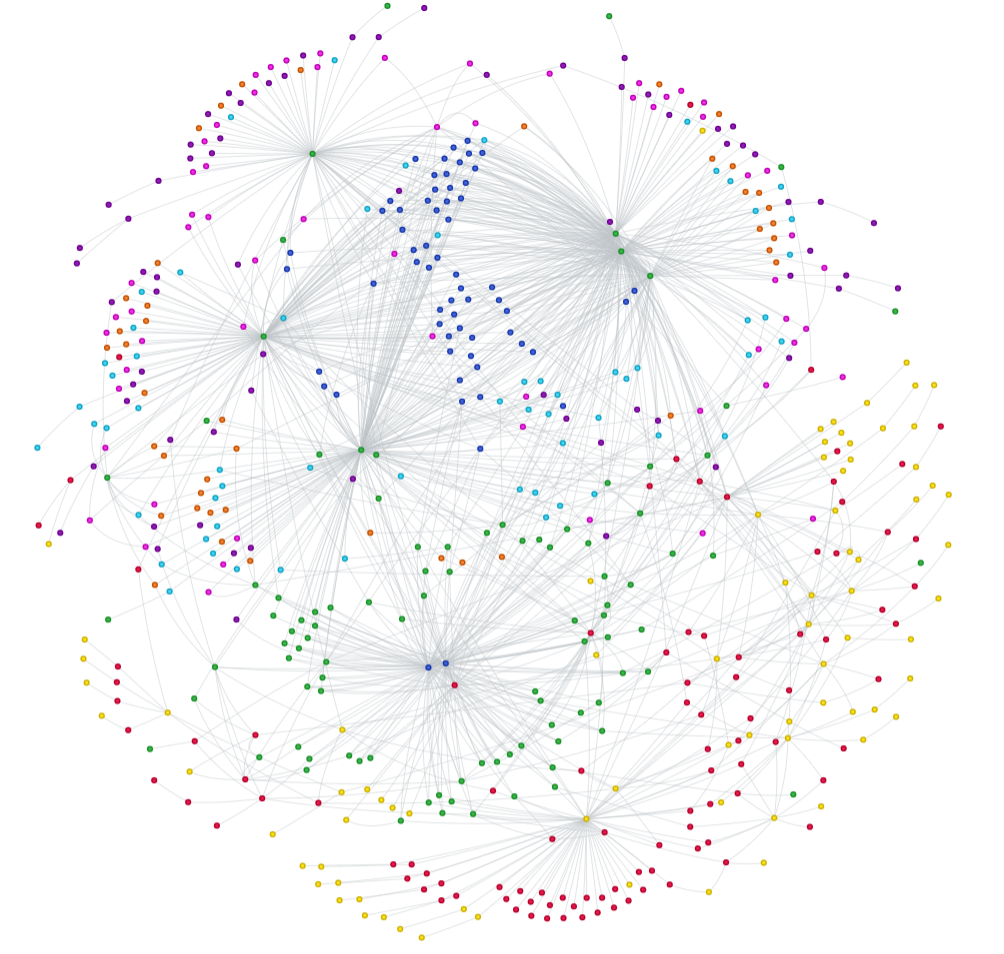
\includegraphics[width=0.48\linewidth]{Figures/NACC-DementiaHKG.png}}\hfill
        \subfloat[ADNI]{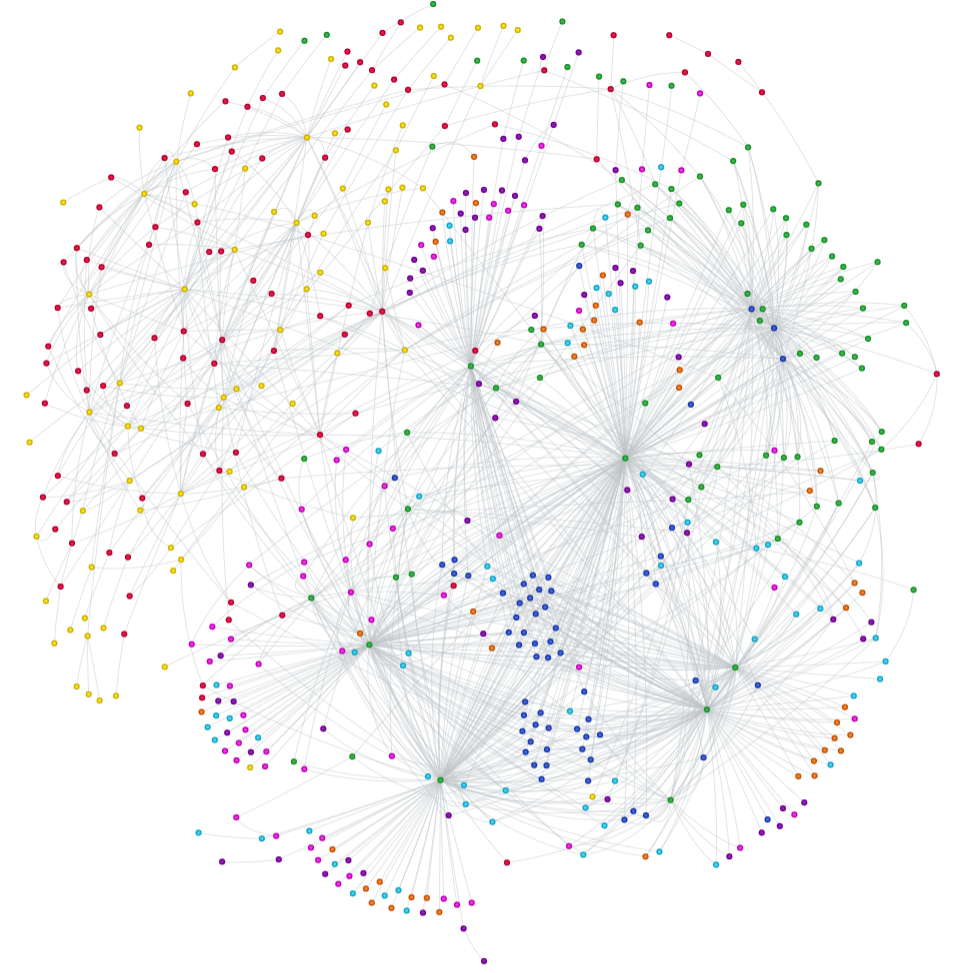
\includegraphics[width=0.48\linewidth]{Figures/ADNI-DementiaHKG.png}}\\
        \subfloat[PPMI]{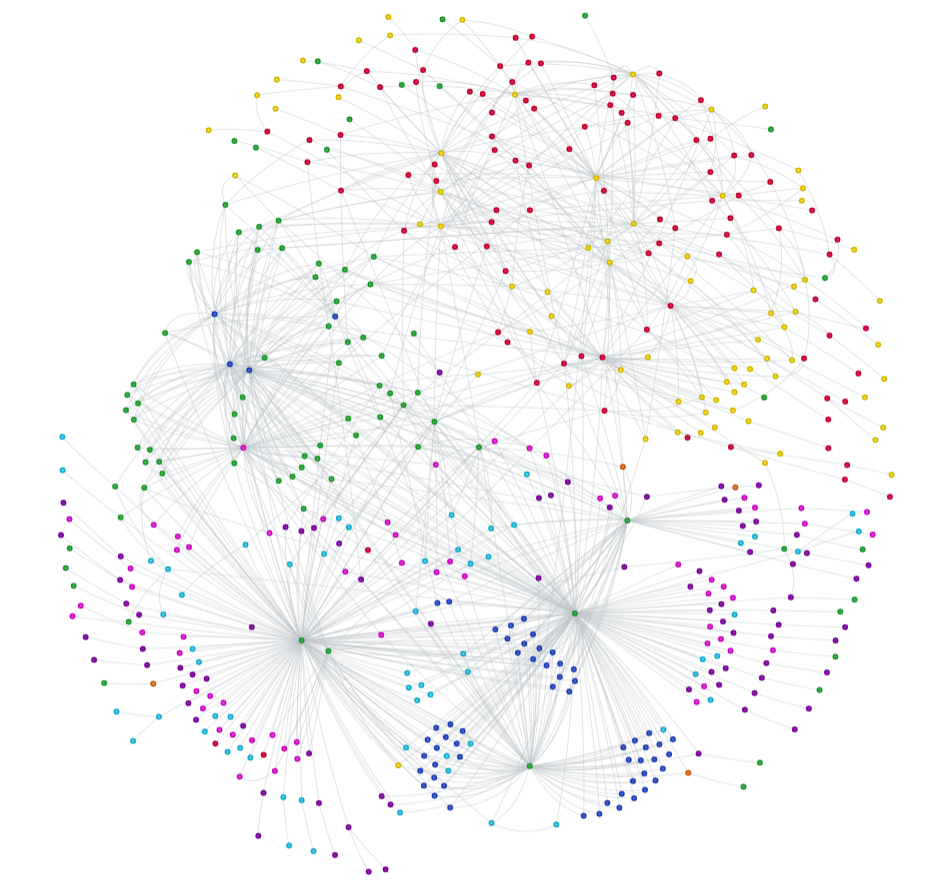
\includegraphics[width=0.48\linewidth]{Figures/PPMI-DementiaHKG.png}}\hfill
        \subfloat[AIBL]{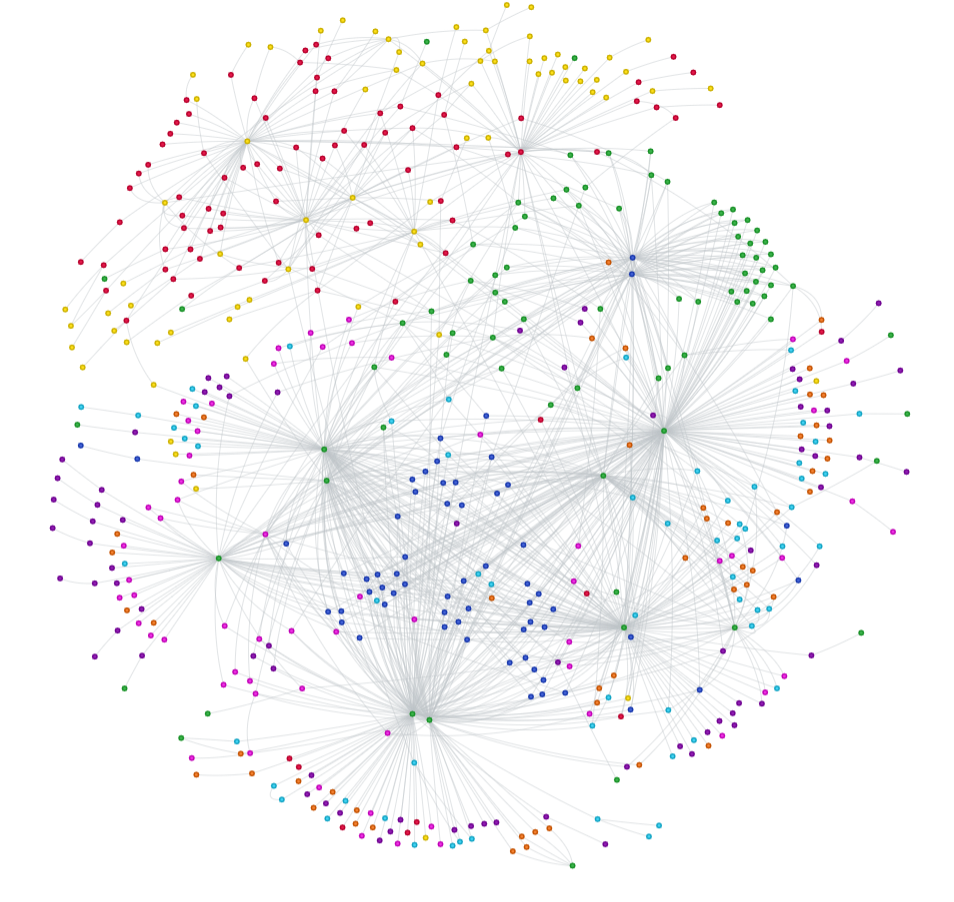
\includegraphics[width=0.48\linewidth]{Figures/AIBL-DementiaHKG.png}}
        \caption{Visualization of DemRKG across datasets: integrating multi-dimensional microscopic entities such as genes, proteins, and diseases.}
        \label{fig:dementia_viz}
    \end{figure}




\subsection{Performance Comparison}

   \begin{table*}[htbp]
\centering
\caption{Performance comparison of different methods on the AIBL, ADNI, NACC, and PPMI benchmarks}
\label{tab:performance_comparison}
\renewcommand{\arraystretch}{1.2} 
\begin{tabular}{llcccccc}
\toprule
\multirow{2}{*}{\textbf{Dataset}} & \multirow{2}{*}{\textbf{Metric}} & \textbf{MM-Trans} & \textbf{MM-Trans} & \textbf{AlignMamba} & \textbf{CAMera} & \textbf{KGT} & \textbf{KAMT} \\
 &  & \textbf{(Bi-modal)} & \textbf{(Tri-modal)} & \textbf{(Tri-modal)} & \textbf{(Tri-modal)} & \textbf{(TransE)} & \textbf{(DemRKG)} \\
\midrule
\multirow{5}{*}{\rotatebox{90}{AIBL}} 
& Accuracy  & 0.5402 $\pm$ 0.0423 & 0.4816 $\pm$ 0.0311 & 0.6204 $\pm$ 0.1238 & 0.6449 $\pm$ 0.1076 & 0.6843 $\pm$ 0.0387 & \textbf{0.8289 $\pm$ 0.0101} \\
& Precision & 0.3704 $\pm$ 0.0542 & 0.4806 $\pm$ 0.0416 & 0.6770 $\pm$ 0.1151 & 0.6692 $\pm$ 0.0732 & 0.5283 $\pm$ 0.1378 & \textbf{0.6977 $\pm$ 0.0253} \\
& Recall    & 0.3725 $\pm$ 0.0458 & 0.4474 $\pm$ 0.0384 & 0.6120 $\pm$ 0.1302 & 0.6462 $\pm$ 0.1114 & 0.4524 $\pm$ 0.0416 & \textbf{0.6912 $\pm$ 0.0253} \\
& F1 Score  & 0.3592 $\pm$ 0.0489 & 0.4146 $\pm$ 0.0603 & 0.5940 $\pm$ 0.1399 & 0.6175 $\pm$ 0.1046 & 0.4419 $\pm$ 0.0305 & \textbf{0.6772 $\pm$ 0.0229} \\
& AUC-ROC   & 0.6173 $\pm$ 0.0312 & 0.4916 $\pm$ 0.0245 & 0.6889 $\pm$ 0.1049 & 0.7292 $\pm$ 0.0514 & 0.7046 $\pm$ 0.0366 & \textbf{0.8660 $\pm$ 0.0259} \\
\midrule
\multirow{5}{*}{\rotatebox{90}{ADNI}} 
& Accuracy  & 0.5210 $\pm$ 0.0991 & 0.5770 $\pm$ 0.0526 & 0.5996 $\pm$ 0.0352 & 0.5676 $\pm$ 0.0263 & 0.6298 $\pm$ 0.0632 & \textbf{0.8299 $\pm$ 0.0112} \\
& Precision & 0.4242 $\pm$ 0.1345 & 0.5709 $\pm$ 0.0760 & 0.5732 $\pm$ 0.0758 & 0.4912 $\pm$ 0.1211 & 0.6011 $\pm$ 0.0848 & \textbf{0.8183 $\pm$ 0.0045} \\
& Recall    & 0.4139 $\pm$ 0.0543 & 0.5351 $\pm$ 0.0441 & 0.4697 $\pm$ 0.0926 & 0.4108 $\pm$ 0.0791 & 0.5633 $\pm$ 0.0734 & \textbf{0.8023 $\pm$ 0.0232} \\
& F1 Score  & 0.3779 $\pm$ 0.0880 & 0.5232 $\pm$ 0.0392 & 0.4350 $\pm$ 0.1224 & 0.3543 $\pm$ 0.1027 & 0.5650 $\pm$ 0.0815 & \textbf{0.8085 $\pm$ 0.0143} \\
& AUC-ROC   & 0.5626 $\pm$ 0.0506 & 0.7493 $\pm$ 0.0163 & 0.7535 $\pm$ 0.0262 & 0.6692 $\pm$ 0.0318 & 0.7696 $\pm$ 0.0620 & \textbf{0.9456 $\pm$ 0.0069} \\
\midrule
\multirow{5}{*}{\rotatebox{90}{NACC}} 
& Accuracy  & 0.5638 $\pm$ 0.0061 & 0.6540 $\pm$ 0.0041 & 0.6193 $\pm$ 0.0060 & 0.5897 $\pm$ 0.0183 & 0.7360 $\pm$ 0.0022 & \textbf{0.8067 $\pm$ 0.0102} \\
& Precision & 0.2474 $\pm$ 0.0558 & 0.5470 $\pm$ 0.0129 & 0.5751 $\pm$ 0.0105 & 0.5565 $\pm$ 0.0516 & 0.6574 $\pm$ 0.0148 & \textbf{0.7674 $\pm$ 0.0126} \\
& Recall    & 0.3364 $\pm$ 0.0046 & 0.5285 $\pm$ 0.0084 & 0.4561 $\pm$ 0.0259 & 0.3679 $\pm$ 0.0320 & 0.6387 $\pm$ 0.0068 & \textbf{0.7395 $\pm$ 0.0180} \\
& F1 Score  & 0.2591 $\pm$ 0.0153 & 0.4962 $\pm$ 0.0080 & 0.4540 $\pm$ 0.0459 & 0.3060 $\pm$ 0.0498 & 0.6302 $\pm$ 0.0221 & \textbf{0.7486 $\pm$ 0.0150} \\
& AUC-ROC   & 0.5695 $\pm$ 0.0111 & 0.7020 $\pm$ 0.0034 & 0.5981 $\pm$ 0.0366 & 0.5034 $\pm$ 0.0375 & 0.8242 $\pm$ 0.0031 & \textbf{0.9274 $\pm$ 0.0042} \\
\midrule
\multirow{5}{*}{\rotatebox{90}{PPMI}} 
& Accuracy  & 0.3227 $\pm$ 0.0564 & 0.4212 $\pm$ 0.0581 & 0.4927 $\pm$ 0.0462 & 0.3788 $\pm$ 0.1291 & 0.3446 $\pm$ 0.0637 & \textbf{0.6185 $\pm$ 0.0125} \\
& Precision & 0.1501 $\pm$ 0.0485 & 0.2653 $\pm$ 0.0494 & 0.4027 $\pm$ 0.1536 & 0.2818 $\pm$ 0.1715 & 0.3575 $\pm$ 0.0869 & \textbf{0.6084 $\pm$ 0.0621} \\
& Recall    & 0.2551 $\pm$ 0.0418 & 0.3647 $\pm$ 0.0631 & 0.4612 $\pm$ 0.0565 & 0.3390 $\pm$ 0.1108 & 0.3264 $\pm$ 0.0493 & \textbf{0.5462 $\pm$ 0.0084} \\
& F1 Score  & 0.1812 $\pm$ 0.0457 & 0.2651 $\pm$ 0.0709 & 0.4101 $\pm$ 0.1117 & 0.2291 $\pm$ 0.1258 & 0.3007 $\pm$ 0.0553 & \textbf{0.5166 $\pm$ 0.0182} \\
& AUC-ROC   & 0.5345 $\pm$ 0.0222 & 0.6740 $\pm$ 0.0827 & 0.6444 $\pm$ 0.1027 & 0.6580 $\pm$ 0.1548 & 0.5842 $\pm$ 0.0631 & \textbf{0.8308 $\pm$ 0.0075} \\
\bottomrule
\end{tabular}
\end{table*}

    As shown in \cref{tab:performance_comparison}, the impact of injecting KG signals is dataset-dependent for vanilla KG encoders, but becomes consistently beneficial under our knowledge-guided design. Specifically, the translation-based baseline KGT (TransE)~\cite{chen2022hybrid,niu2024ehrknowgen} can improve over MM-Trans (Tri-modal)~\cite{chen2021iccv-multimodal-a} on the text-rich NACC benchmark (F1: +0.1340; Acc: +0.0820), yet it degrades on the more challenging four-class PPMI task (Acc: 0.4212 $\rightarrow$ 0.3446), suggesting potential negative transfer when KG embeddings are not aligned with multimodal clinical evidence.

    We further include two recent tri-modal baselines, AlignMamba~\cite{li2025alignmamba} and CAMera~\cite{hu2025camera} , which strengthen the non-KG comparison. Despite their improvements over MM-Trans in several settings, KAMT (DemRKG) achieves the best overall and most stable performance across all four datasets, yielding clear margins on both class-sensitive metrics (F1/Recall) and threshold-free AUC-ROC (e.g., ADNI AUC-ROC: 0.9456 vs. 0.7535/0.6692; AIBL Acc: 0.8289 vs. 0.6204/0.6449 for AlignMamba/CAMera). These results support that (i) DemRKG provides higher-quality relational representations tailored to the dementia diagnosis context, and (ii) knowledge-aware cross-attention with masking effectively constrains cross-modal interactions, improving optimization stability and generalization.


\subsection{Ablation Study}

This section aims to analyze the specific contributions of knowledge graphs derived from different sources and construction methods to the overall multimodal diagnostic performance.

\subsubsection{Ablation on Knowledge Fusion Mechanisms and Strategies}

    To explore the impact of different knowledge graphs within the KAMT architecture, we compare the core metrics of three configurations across various clinical cases: private domain knowledge guidance (CustomKG), an unrefined external knowledge base (PrimeKG), and our proposed relational graph (DemRKG). For three kinds of domain knowledge representations, the comprehensive evaluation of was presented in Table \ref{tab:comprehensive_performance}.

\begin{table}[htbp]
    \centering
    \caption{Ablation study of tri-modal learning guided by different KGs under the KAMT architecture.}
    \label{tab:comprehensive_performance}
    \renewcommand{\arraystretch}{1.2}
    \resizebox{\columnwidth}{!}{%
    \begin{tabular}{c|c|ccc}
        \toprule
        Data & Metric & CustomKG & PrimeKG & \textbf{DemRKG} \\
        \hline
        \multirow{5}{*}{\rotatebox{90}{AIBL}} 
        & Accuracy & 0.7783 $\pm$ 0.0138 & 0.8193 $\pm$ 0.0148 & \textbf{0.8289 $\pm$ 0.0101} \\
        & Precision & 0.6686 $\pm$ 0.0254 & 0.6586 $\pm$ 0.0165 & \textbf{0.6977 $\pm$ 0.0253} \\
        & Recall & 0.5839 $\pm$ 0.0706 & 0.6597 $\pm$ 0.0177 & \textbf{0.6912 $\pm$ 0.0253} \\
        & F1 score & 0.5898 $\pm$ 0.0545 & 0.6476 $\pm$ 0.0090 & \textbf{0.6772 $\pm$ 0.0229} \\
        & AUROC & 0.8091 $\pm$ 0.0181 & 0.8455 $\pm$ 0.0077 & \textbf{0.8660 $\pm$ 0.0259} \\
        \hline
        \multirow{5}{*}{\rotatebox{90}{ADNI}} 
        & Accuracy & 0.7239 $\pm$ 0.0315 & 0.7671 $\pm$ 0.0254 & \textbf{0.8299 $\pm$ 0.0112} \\
        & Precision & 0.5318 $\pm$ 0.1213 & 0.7652 $\pm$ 0.0594 & \textbf{0.8183 $\pm$ 0.0045} \\
        & Recall & 0.6284 $\pm$ 0.1018 & 0.7095 $\pm$ 0.0768 & \textbf{0.8023 $\pm$ 0.0232} \\
        & F1 score & 0.5735 $\pm$ 0.1092 & 0.6941 $\pm$ 0.0835 & \textbf{0.8085 $\pm$ 0.0143} \\
        & AUROC & 0.8957 $\pm$ 0.0245 & 0.9283 $\pm$ 0.0059 & \textbf{0.9456 $\pm$ 0.0069} \\
        \hline
        \multirow{5}{*}{\rotatebox{90}{NACC}} 
        & Accuracy & 0.7875 $\pm$ 0.0095 & 0.7970 $\pm$ 0.0087 & \textbf{0.8067 $\pm$ 0.0102} \\
        & Precision & 0.7439 $\pm$ 0.0094 & 0.7364 $\pm$ 0.0148 & \textbf{0.7674 $\pm$ 0.0126} \\
        & Recall & 0.7154 $\pm$ 0.0183 & 0.7330 $\pm$ 0.0156 & \textbf{0.7395 $\pm$ 0.0180} \\
        & F1 score & 0.7227 $\pm$ 0.0170 & 0.7372 $\pm$ 0.0163 & \textbf{0.7486 $\pm$ 0.0150} \\
        & AUROC & 0.9128 $\pm$ 0.0030 & 0.9209 $\pm$ 0.0025 & \textbf{0.9274 $\pm$ 0.0042} \\
        \hline
        \multirow{5}{*}{\rotatebox{90}{PPMI}} 
        & Accuracy & 0.4892 $\pm$ 0.0768 & 0.5877 $\pm$ 0.0329 & \textbf{0.6185 $\pm$ 0.0125} \\
        & Precision & 0.4883 $\pm$ 0.1659 & 0.4738 $\pm$ 0.0959 & \textbf{0.6084 $\pm$ 0.0621} \\
        & Recall & 0.4379 $\pm$ 0.0722 & 0.5002 $\pm$ 0.0394 & \textbf{0.5462 $\pm$ 0.0084} \\
        & F1 score & 0.4025 $\pm$ 0.0765 & 0.4522 $\pm$ 0.0559 & \textbf{0.5166 $\pm$ 0.0182} \\
        & AUROC & 0.7033 $\pm$ 0.0628 & 0.8285 $\pm$ 0.0156 & \textbf{0.8308 $\pm$ 0.0075} \\
        \bottomrule
    \end{tabular}}
\end{table}

    As illustrated by \ref{tab:comprehensive_performance}, after introducing external domain knowledge, PrimeKG's prediction performance is generally better than CustomKG. The external knowledge base covers multi-dimensional medical consensus, including disease targets and gene expression, effectively compensating for the limitations of semantic association in single internal diagnostic records.

    In the selected cases, the distilled DemRKG representations have achieved the best metrics. Ablation experiments verified that the refined relational knowledge graph DemRKG can effectively eliminate redundant connections between medical entities and maintain the performance of diagnostic models even in complex cases.

\subsubsection{Validation of Architectural Generalization and Prediction Stability}

    To isolate the contribution of our network design from the knowledge graph, we introduce a baseline model, KAMP (Knowledge-Aware Multimodal Perceiver), which relies on a latent variable bottleneck mechanism. Both architectures are evaluated under identical conditions, integrating the domain-specific DemRKG. The comparative performance across multicenter datasets is detailed in Table \ref{tab:arch_compare}.

\begin{table}[htbp]
    \centering
    \caption{Performance comparison across architectures integrating DemRKG}
    \label{tab:arch_compare}
    \renewcommand{\arraystretch}{1.2}
    \resizebox{\columnwidth}{!}{%
    \begin{tabular}{c|c|cc}
        \toprule
        Data & Metric & KAMT (DemRKG) & KAMP (DemRKG) \\
        \hline
        \multirow{5}{*}{\rotatebox{90}{AIBL}} 
        & Accuracy & \textbf{0.8289 $\pm$ 0.0101} & 0.8193 $\pm$ 0.0108 \\
        & Precision & \textbf{0.6977 $\pm$ 0.0253} & 0.6899 $\pm$ 0.0232 \\
        & Recall & \textbf{0.6912 $\pm$ 0.0253} & 0.6890 $\pm$ 0.0218 \\
        & F1 score & 0.6772 $\pm$ 0.0229 & \textbf{0.6804 $\pm$ 0.0188} \\
        & AUROC & 0.8660 $\pm$ 0.0259 & \textbf{0.8689 $\pm$ 0.0079} \\
        \hline
        \multirow{5}{*}{\rotatebox{90}{ADNI}} 
        & Accuracy & \textbf{0.8299 $\pm$ 0.0112} & 0.8254 $\pm$ 0.0060 \\
        & Precision & \textbf{0.8183 $\pm$ 0.0045} & 0.8148 $\pm$ 0.0138 \\
        & Recall & 0.8023 $\pm$ 0.0232 & \textbf{0.8038 $\pm$ 0.0186} \\
        & F1 score & \textbf{0.8085 $\pm$ 0.0143} & 0.8063 $\pm$ 0.0055 \\
        & AUROC & 0.9456 $\pm$ 0.0069 & \textbf{0.9477 $\pm$ 0.0033} \\
        \hline
        \multirow{5}{*}{\rotatebox{90}{NACC}} 
        & Accuracy & \textbf{0.8067 $\pm$ 0.0102} & 0.7815 $\pm$ 0.0064 \\
        & Precision & \textbf{0.7674 $\pm$ 0.0126} & 0.7345 $\pm$ 0.0106 \\
        & Recall & \textbf{0.7395 $\pm$ 0.0180} & 0.7071 $\pm$ 0.0133 \\
        & F1 score & \textbf{0.7486 $\pm$ 0.0150} & 0.7162 $\pm$ 0.0133 \\
        & AUROC & \textbf{0.9274 $\pm$ 0.0042} & 0.9113 $\pm$ 0.0028 \\
        \hline
        \multirow{5}{*}{\rotatebox{90}{PPMI}} 
        & Accuracy & \textbf{0.6185 $\pm$ 0.0125} & 0.5661 $\pm$ 0.0265 \\
        & Precision & \textbf{0.6084 $\pm$ 0.0621} & 0.5222 $\pm$ 0.0448 \\
        & Recall & \textbf{0.5462 $\pm$ 0.0084} & 0.4962 $\pm$ 0.0269 \\
        & F1 score & \textbf{0.5166 $\pm$ 0.0182} & 0.4736 $\pm$ 0.0261 \\
        & AUROC & \textbf{0.8308 $\pm$ 0.0075} & 0.8018 $\pm$ 0.0189 \\
        \bottomrule
    \end{tabular}}
\end{table}

    In benchmark characterized by a lower density of textual modalities, both KAMT and KAMP architectures have exhibited comparable diagnostic capabilities. As demonstrated in Table \ref{tab:arch_compare}, their metrics are nearly equivalent on the AIBL and ADNI datasets. However, the architectural superiority of KAMT becomes pronounced when handling highly heterogeneous, high-dimensional phenotypic data. This performance gap is directly attributable to the handling of information bottlenecks. KAMP forces complex fine-grained features into a compressed low-dimensional latent space, which inevitably degrades data fidelity. Conversely, KAMT employs a modality-aware strategy that preserves the original distribution of the underlying clinical data, preventing critical signal loss.

\begin{comment}

%\subsubsection{Discussion on the Multimodal Diagnostic Paradigm}
The comprehensive ablation studies systematically validate the efficacy of the "diagnostic knowledge graph guidance combined with multimodal data" paradigm for complex brain disease diagnosis. The core mechanisms driving this performance improvement can be condensed into three key aspects:

\begin{itemize}
    \item \textbf{Dynamic Regularization via Relational Graph (DemRKG):} By tailoring the broad biomedical consensus of PrimeKG against private domain datasets, DemRKG achieves a critical balance between knowledge breadth and depth. It acts as a dynamic regularizer, constraining the multimodal learning (MML) process and preventing the noise inherent in unrefined external databases.
    
    \item \textbf{Implicit Constraint via Cross-Attention Synergy:} KAMT abandons the brute-force feature stacking of conventional MML. Through a cross-self-attention module paired with a mask operation layer, DemRKG tokens serve as an implicit constraint, guiding the network to actively discover optimal alignments between general pathological relationships and specific clinical signals.
    
    \item \textbf{High-Fidelity Modality Preservation:} Unlike Perceiver-based architectures (KAMP) that compress inputs into a low-dimensional latent bottleneck, KAMT preserves the original distribution of the data. It enables fine-grained interactions between external knowledge and specific inputs—such as Bio clinical scales, EHR demographics, and 3D-CNN preprocessed MRI features—capturing the subtle pathologies essential for accurate diagnosis.
\end{itemize}
\end{comment}


\subsection{Investigation of Clinical Knowledge Representations}

    Illustrated in Table \ref{tab:comprehensive_performance}, the distilled \textcolor{blue}{DemRKG} leads to a secondary leap in performance. Based on the universal convergence improvements observed, we identify the following core mechanisms:

    % \subsubsection{Stabilization of Optimization Landscape (Global Mechanism)}
    
    The primary contribution of the \textcolor{blue}{KGE learning} is its role as a powerful \textbf{Regularizer}. In medical multimodal learning, the feature space is often high-dimensional yet sparse, creating a highly volatile loss landscape. The injection of pre-trained KG embeddings (DistMult/\textcolor{blue}{DemRKG}) provides a stable ``skeleton'' (manifold) for the feature space. This significantly reduces the search space for the Multimodal Transformer, ensuring consistent convergence across all datasets (ADNI, PPMI, NACC, AIBL), preventing the model from collapsing into random guessing.

    % \subsubsection{Semantic Anchoring Effect}

    Purely data-driven models may treat clinical attributes as isolated tokens. By mapping attributes (e.g., \texttt{upd2315a}) to standardized entities in \textcolor{blue}{DemRKG} (e.g., \texttt{Symptom:Rest\_Tremor}), KAMT injects an explicit inductive bias, encouraging representations to align with clinically meaningful semantics. In addition, hierarchical instantiation ($\text{Patient} \to \text{Level} \to \text{Concept}$) links patients with different symptom severity through shared parental concepts, which helps reduce overfitting in limited sample sizes.

\section{Summary and Discussion}

    % \subsubsection{Dynamic Regularization with Efficient Structural Priors}

    As demonstrated in \cref{fig:accuracy_boxplot}, the purely data-driven baseline (MM-Trans) exhibits larger performance variance and more outliers across four independent cohorts, suggesting vulnerability to spurious cross-modal shortcuts in ambiguous cases. KAMT mitigates this issue by introducing refined DemRKG tokens and applying masking within cross-attention as an implicit, sample-adaptive constraint, thereby stabilizing feature optimization and improving diagnostic reliability. To keep this structural knowledge computationally tractable, we use DistMult-style bilinear scoring to encode latent interactions among biological entities while reducing redundant computation, providing compact yet informative structural priors for regularization.

\begin{figure}[!t]
    \centering
    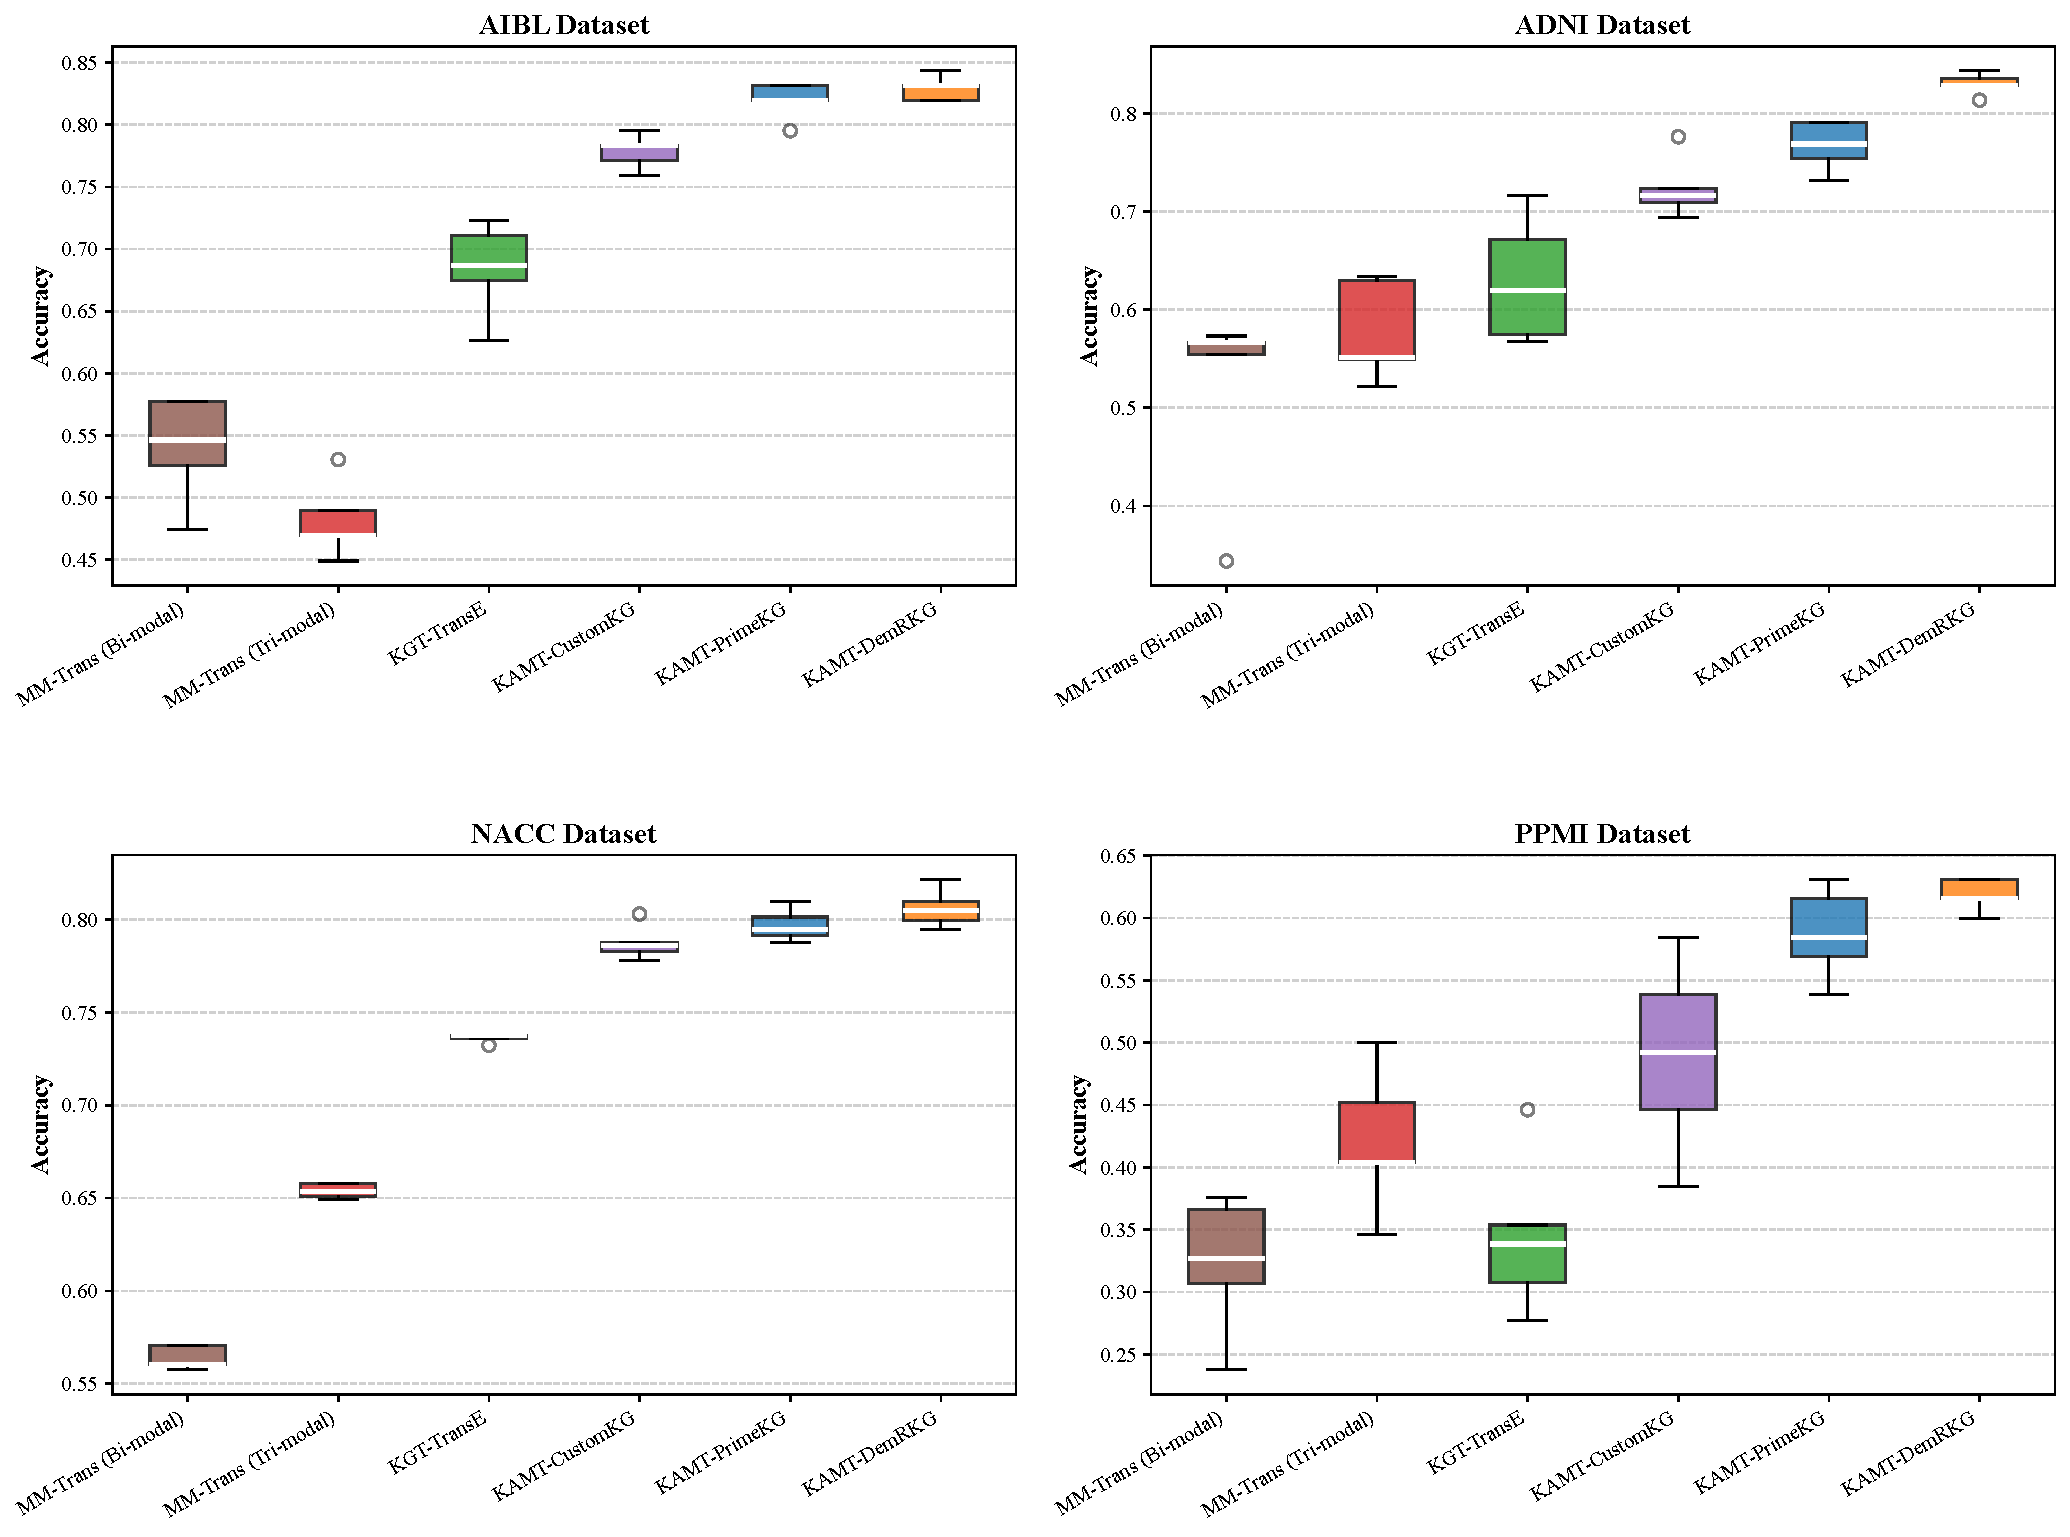
\includegraphics[width=0.9\linewidth]{Figures/箱型图-EN.pdf}
    \caption{Boxplot of prediction accuracy distribution across four independent cohorts.}
    \label{fig:accuracy_boxplot}
\end{figure}

\subsubsection{Semantic Preservation in Fine-Grained Alignment}

    Fine-grained diagnosis can degrade when architectures impose aggressive compression (e.g., information bottlenecks), especially for dense text or detailed clinical scales (e.g., demographics in EHR and UPDRS in BioMarker). KAMT therefore enforces strict dimensional matching between Queries and Keys, enabling a point-to-point alignment between clinical observations and DemRKG nodes. Meanwhile, the knowledge injection is coupled with the energy-constrained refinement in \cref{eq:energy_min}, which helps keep the aligned representations consistent with observed clinical measurements while preserving fine-grained semantics.

\subsubsection{Clinical Limitations and Real-World Applicability}

Real-world deployment is still limited by reliance on complete cross-sectional snapshots, partial loss of topological detail in the current structural representation, and the lack of explicit causal reasoning paths. Future work will explore missing-modality-aware longitudinal modeling, higher-dimensional graph representations to preserve edge-level semantics, and path-tracking strategies to reconstruct interpretable reasoning chains.

%\section{Data availability}

    %\textcolor{blue}{The Parkinson’s Progression Markers Initiative (PPMI, http://www.ppmi-info.org/) database and the Parkinson’s Disease Biomarkers Program (PDBP, https://pdbp.ninds.nih.gov/) database used in this study are both accessible through AMP-PD (https://amp-pd.org/). To access clinical and omics data at the AMP-PD Tier 2 level, users are required to complete a data use agreement and submit an online application.}
	

%\section*{Code availability}

	%This M$^2$STGAT method is implemented in Python and available in Github (https://github.com/ZJ-BMDmining/M2DGAT).


    
%\section*{Acknowledgment}

	%This work is sponsored by National Natural Science Foundation of China(62302455, 62172369), Special Support Plan for High-level Talents in Zhejiang Province(2021R52019) and Natural Science Foundation of Zhejiang Province, China(LQ24F030007).
	
	

%\section*{References}
\bibliographystyle{IEEEtran}
\bibliography{references.bib}




\vfill

\end{document}


